\documentclass[
	% -- op\c{c}\~{o}es da classe memoir --
	12pt,				% tamanho da fonte
	openright,			% cap\'{\i}tulos come\c{c}am em p\'{a}g \'{\i}mpar (insere p\'{a}gina vazia caso preciso)
	oneside,			% para impress\~{a}o em recto e verso. Oposto a oneside
	a4paper,			% tamanho do papel.
	english,			% idioma adicional para hifeniza\c{c}\~{a}o
	french,				% idioma adicional para hifeniza\c{c}\~{a}o
	spanish,			% idioma adicional para hifeniza\c{c}\~{a}o
	brazil,				% o \'{u}ltimo idioma \'{e} o principal do documento
	]{abntex2}

\usepackage{lmodern}			% Usa a fonte Latin Modern
\usepackage[T1]{fontenc}		% Selecao de codigos de fonte.
\usepackage[utf8]{inputenc}		% Codificacao do documento (convers\~{a}o autom\'{a}tica dos acentos)
\usepackage{indentfirst}		% Indenta o primeiro par\'{a}grafo de cada se\c{c}\~{a}o.
\usepackage{color}				% Controle das cores
\usepackage{graphicx}			% Inclus\~{a}o de gr\'{a}ficos
\usepackage{microtype} 			% para melhorias de justifica\c{c}\~{a}o
\usepackage{float}
\usepackage{adjustbox}
\usepackage{mwe} % new package from Martin scharrer
\usepackage{caption}
\usepackage{cellspace}
\usepackage{gensymb}

\setlength\cellspacetoplimit{4pt}
\setlength\cellspacebottomlimit{4pt}



\usepackage{adjustbox}
\restylefloat{table}

\setcounter{topnumber}{5}
\setcounter{bottomnumber}{5}
\setcounter{totalnumber}{5}
\usepackage[section]{placeins}
\usepackage{multicol}
\usepackage{multirow}
\usepackage{lipsum}
\usepackage[brazilian,hyperpageref]{backref}	 % Paginas com as cita\c{c}\~{o}es na bibl
\usepackage[alf]{abntex2cite}	% Cita\c{c}\~{o}es padr\~{a}o ABNT
\usepackage[utf8]{inputenc}
\usepackage{amsmath,amsfonts,amssymb}

% Configura\c{c}\~{o}es do pacote backref
% Usado sem a op\c{c}\~{a}o hyperpageref de backref
\renewcommand{\backrefpagesname}{Citado na(s) p\'{a}gina(s):~}
% Texto padr\~{a}o antes do n\'{u}mero das p\'{a}ginas
\renewcommand{\backref}{}
% Define os textos da cita\c{c}\~{a}o
\renewcommand*{\backrefalt}[4]{
	\ifcase #1 %
		Nenhuma cita\c{c}\~{a}o no texto.%
	\or
		Citado na p\'{a}gina #2.%
	\else
		Citado #1 vezes nas p\'{a}ginas #2.%
	\fi}%
% ---

% ---
% Informa\c{c}\~{o}es de dados para CAPA e FOLHA DE ROSTO
% ---
\titulo{Relat\'{o}rio IX}
\autor{Francisco Edson Birimba Brito \\ Gisele Ribeiro Gomes \\ Gabriel Marques de Silva Abreu \\ Matheus Paolo dos Anjos Mour\~{a}o \\ Paulo Chaves dos Santos J\'{u}nior}
\local{Rio Branco, Acre}
\data{2017}
\instituicao{%
  Universidade Federal do Acre - UFAC
  \par
  Bacharelado em Engenharia El\'{e}trica
  \par
  Laborat\'{o}rio de Eletr\^{o}nica I}
\tipotrabalho{Relat\'{o}rio t\'{e}cnico}
% O preambulo deve conter o tipo do trabalho, o objetivo,
% o nome da institui\c{c}\~{a}o e a \'{a}rea de concentra\c{c}\~{a}o
\preambulo{Relat\'{o}rio de Laborat\'{o}rio de Eletr\^{o}nica I, entregue para a composi\c{c}\~{a}o parcial da nota da N1.
Orientador : Elmer Osman Hancco}
% ---

% ---
% Configura\c{c}\~{o}es de apar\^{e}ncia do PDF final

% alterando o aspecto da cor azul
\definecolor{blue}{RGB}{41,5,195}

% informa\c{c}\~{o}es do PDF
\makeatletter
\hypersetup{
     	%pagebackref=true,
		pdftitle={\@title},
		pdfauthor={\@author},
    	pdfsubject={\imprimirpreambulo},
	    pdfcreator={LaTeX with abnTeX2},
		pdfkeywords={abnt}{latex}{abntex}{abntex2}{relat\'{o}rio t\'{e}cnico},
		colorlinks=true,       		% false: boxed links; true: colored links
    	linkcolor=black,          	% color of internal links
    	citecolor=blue,        		% color of links to bibliography
    	filecolor=magenta,      		% color of file links
		urlcolor=blue,
		bookmarksdepth=4
}
\makeatother

\setlength{\parindent}{1.3cm}

\setlength{\parskip}{0.2cm}  % tente tamb\'{e}m \onelineskip

\makeindex

\begin{document}

\selectlanguage{brazil}

\frenchspacing

\imprimircapa

\imprimirfolhaderosto*

\setlength{\absparsep}{18pt} % ajusta o espa\c{c}amento dos par\'{a}grafos do resumo
 \begin{resumo}
A prática presente baseia-se na montagem dos circuitos com o transistor $ 2N3391 $, sendo simulado com a utilização do software MULTISIM, aplicado um gerador de funções com uma tensão de $ 1,0mV $ e frequência $ 1 kHz $ e com o ganho gerado, analisamos a relação com a frequência. Utilizando o \textit{diagrama de Bode}, sendo uma forma de caracterizar sinais no domínio da frequência. E apresentação de conceitos de filtros, apresentando um exemplo prático desta aplicação. \\
 \noindent
 \textbf{Palavras-chaves}:bode plots, frequência, amplificador
\end{resumo} 


 \setlength{\absparsep}{18pt} % ajusta o espa\c{c}amento dos par\'{a}grafos do resumo
\begin{resumo}[Abstract]
In this report it was studied the implementation of an amplifier circuit with common emitter configuration as well as analysis of the operating points and variables CC and CA of the circuit. The comparison of theoretically obtained values and experimental values was also performed.\\
\noindent
\textbf{Keyword}: amplifier, common emitter, AC
\end{resumo} 


\pdfbookmark[0]{\contentsname}{toc}
\tableofcontents*

\cleardoublepage

\textual
\chapter*[Introdu\c{c}\~{a}o]{Introdu\c{c}\~{a}o}
\addcontentsline{toc}{chapter}{Introdu\c{c}\~{a}o}

	Neste relatório temos como objetivo a familiarização a resposta em frequência e o uso do diagrama de bode, onde trabalhamos no $ 1^\circ $ e $ 2^\circ $ estágio e depois com os dois ao mesmo tempo do amplificador, sendo usado o transistor $ 2N3391 $. Analisando o ganho do amplificador e depois relacionando com a frequência. Apresentando também conceitos de filtro passa baixa, passa alta, rejeita faixa e passa faixa.
\setcounter{topnumber}{5}
\setcounter{bottomnumber}{5}
\setcounter{totalnumber}{5}

\chapter{Procedimentos e resultados}

%\centerline{\begin{minipage}[c]{\textwidth}
%		\centering
%		\noindent
%		\captionof{figure}{Transistor bipolar atuando como chave}
%		\begin{figure}
%			\centering
%			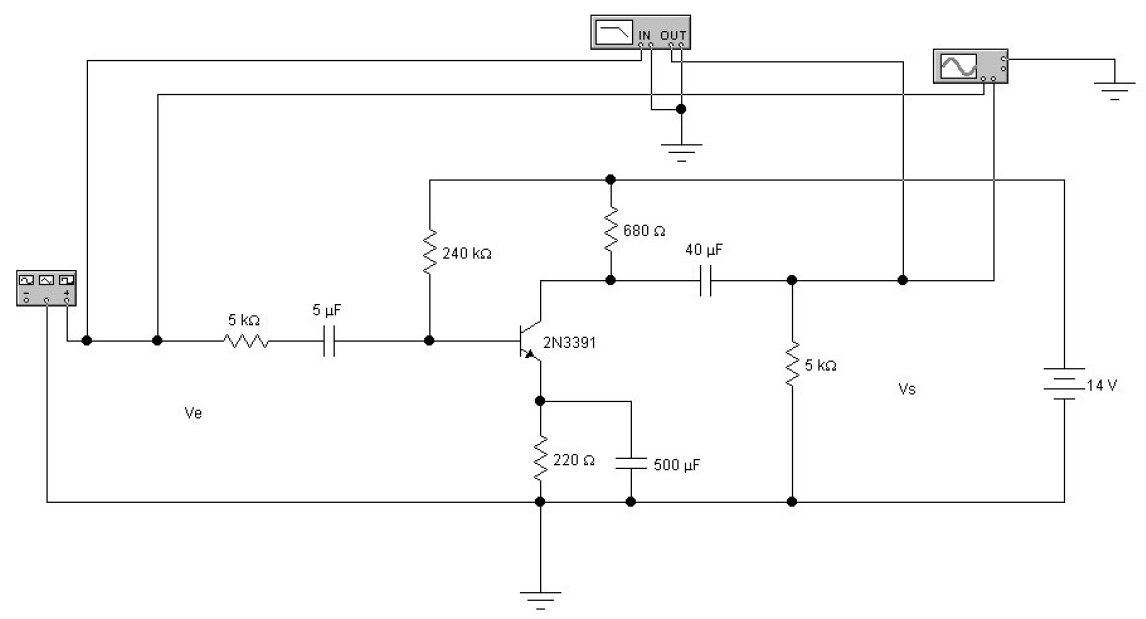
\includegraphics[width=0.7\linewidth]{Imagens/Figura1.jpg}
%			\caption{}
%			\end{figure}
%		\legend{Fonte: Produzido pelos autores}
%		\label{Figura1}
%\end{minipage}}
% DAR CTRL + U PARA TIRAR O COMENTÁRIO
	
	ADD a figura 1

\begin{enumerate}
	\item Monte o circuito da Figura 1 com transistor bipolar atuando na condição de saturação. Meça as variáveis mostradas na Tabela \ref{Tabela1} e calcule os erros percentuais:


	\centerline{\begin{minipage}[c]{\textwidth}
	\centering
	\noindent
	\captionof{table}{Valores teóricos e práticos na condição de saturação}
\begin{tabular}{cccc}
	\toprule
	Variável & Valor teórico & Valor prático & Erro (\%) \\
	\midrule \midrule
	$I_{C}$ (SAT) & 9,86 mA & 10,15 mA & 2,96 \\
	\midrule
	$I_{B}$ (SAT) & 30,42 $\mu A$ & 31,3 $\mu A$ & 2,87 \\
	\midrule
	$\beta_{cc}$ (SAT) & 324 &  324,28 & 0,09 \\
	\midrule
	$VCE$ (SAT) & 9,89 mA & 10,15 mA & 2,85 \\
	\midrule
	\bottomrule
\end{tabular}%
\legend{Fonte: Produzido pelos autores}
\label{Tabela1}
\end{minipage}}


	\item Monte o circuito da Figura 1 com o transitor bipolar atuando na condição de corte. Meça as variáveis mostradas na Tabela \ref{Tabela2} e calcle os erros percentuais.


	\centerline{\begin{minipage}[c]{\textwidth}
	\centering
	\noindent
	\captionof{table}{Valores teóricos e práticos na condição de corte}
\begin{tabular}{cccc}
	\toprule
	Variável & Valor teórico & Valor prático & Erro (\%) \\
	\midrule \midrule
	$I_{C}$ (CORTE) & 9,86 mA & 10,15 mA & 2,96 \\
	\midrule
	$I_{B}$ (CORTE) & 30,42 $\mu A$ & 31,3 $\mu A$ & 2,87 \\
	\midrule
	$VCE$ (SAT) & 9,89 mA & 10,15 mA & 2,85 \\
	\midrule
	\bottomrule
\end{tabular}%
\legend{Fonte: Produzido pelos autores}
\label{Tabela2}
\end{minipage}}


	\item Verifique na folha de dados do transistor BC547B os valores de $ V_{CE} $ (SAT) $ V $ e de $ I_C $ (CORTE). Compare com os valores medidos.




	\item Monte o circuito da Figura 2 com transistor bipolar atuando como chave no acionamento de um relé. Verifique o correto funcionamento do circuito.
\end{enumerate}

	
	Add A imagem "TransistorBipolar"
	
Para a simulação usamos o programa Proteus, montando o mesmo esquema da figura anterior, onde usamos um \textit{switch}  para ficamos variando a tensão de entrada na base de $ 0 V $ para $ 15 V $, ficando da seguinte maneira:

	Add a imagem "Imagem 1"

Ao ligamos o circuito, com a base do transistor recebendo aproximadamente $ 0 V $, temos que não há variação no relé, fazendo com que o LED não receba nenhuma corrente, como mostrado na imagem abaixo:

	Add a imagem "Etapa 1"
	
Agora mudando a tensão de entrada da base para $ 15 V $ temos que internamente, uma corrente circula pela bobina, fazendo criar um campo magnético, atraindo assim o contato do relé, fechando assim o circuito do LED, fazendo ele acender. Como mostramos na próxima figura:

	Add a imagem "Etapa 2"
	
Temos assim, que quando cessamos a corrente da bobina, o contato do relé volta para a posição normal, abrindo assim o circuito do LED.

	
	


\chapter{Conclus\~{a}o}
Todo o processo de montagem e teste dos circuitos indicados no relatório, com exceção do passo 7 (que após várias tentativas foram atribuídos erros técnicos aos equipamentos e componentes utilizados, porém segue em anexo uma simulação correta do exercício), seguiram de acordo com o esperado, foram entendidos e montados intuitivamente.
A respeito de discrepâncias entre os valores teóricos e práticos, são devidas a dificuldade do estabelecimento de um beta que seja compatível com o real.
Em sumo, a prática dos conceitos estudados em sala foi edificante, como por exemplo: a aplicação de um transistor para chaveamento.
\postextual

\bibliography{Referencias}




\end{document}
